As explained in the above introduction, Stratum aimed to solve two main inefficiencies of the previous getwork protocol:
\begin{enumerate}
    \item HTTP used as a transport protocol.
    \item Excessive number of job requests made by miners to the pool server due to the absence of an extranonce field to modify during mining activity.
\end{enumerate}

\noindent To solve the first issue, Stratum was developed as <<a line-based protocol using plain TCP socket, with payload encoded as JSON-RPC messages. Client simply opens TCP socket and writes requests to the server in the form of JSON messages finished by the newline character. Every line received by the client is again a valid JSON-RPC fragment containing the response. There's no HTTP overhead involved and there are no hacks like mining extension flags encoded in HTTP headers anymore. But the biggest improvement from HTTP-based getwork is the fact, that server can drive the load by itself, it can send broadcast messages to miners at any time without any long-polling workarounds, load balancing issues and packet storms.>>\cite{braiinsStratumDocs}\\\\
To go into deeper details, Stratum solved the inefficiencies introduced by using HTTP as the transport protocol through the following key solutions:
\begin{itemize}
    \item \textbf{Line-Based Protocol}: Stratum introduced a line-based protocol over plain TCP sockets. Instead of relying on the complexities of HTTP, the communication in Stratum is simplified by sending and receiving messages as lines of text. Each line represents a valid JSON-RPC fragment containing requests or responses.
    \item \textbf{JSON-RPC Encoding}: Stratum encodes the payload of the communication as JSON-RPC messages: JSON provides a lightweight and structured data format that is easy to parse and generate. By utilizing JSON-RPC, Stratum achieves efficient and compact encoding of data, reducing the overall size of the transmitted messages.
    \item \textbf{Direct Socket Connection}: Stratum utilizes direct socket connections between the mining pool server and the miners. This direct communication enables a more efficient data exchange, eliminating the need for the additional overhead and complexities associated with HTTP.
    \item \textbf{Real-time Updates and Push Mechanism}: Stratum introduced a push mechanism for real-time updates. Unlike the previous getwork protocol, where miners had to explicitly request new mining jobs, Stratum allows mining pool servers to proactively push mining jobs to subscribed miners. This eliminates the delay and latency caused by frequent client requests, ensuring that miners are always provided with the correct mining work.
    \item \textbf{Load Management and Broadcast Messages}: Stratum enables mining pool servers to manage the load and send broadcast messages to miners as needed. This eliminates the need for workarounds such as Long Polling and mitigates the issues of load balancing and packet storms that were present in the getwork protocol. The mining server can efficiently control and distribute the workload across the connected miners.
\end{itemize}
By implementing these solutions, Stratum solves the inefficiencies introduced by using HTTP as the transport protocol. The line-based protocol, combined with JSON-RPC encoding and direct socket connections, reduced the communication overhead and improved the efficiency of data transfer. Real-time updates and the push mechanism allowed for immediate job distribution, eliminating the delays caused by explicit client requests.\\\\
To overcome the second getwork inefficiency, Stratum protocol introduced the concept of an \textbf{extranonce} field. The extranonce field is a mutable portion of the coinbase transaction in the block template that miners can modify during the mining process. By allowing miners to modify the extranonce, Stratum expanded the search space for a valid block nonce without requiring frequent job requests to the pool server.\\
With the extranonce field, miners could vary its value while keeping the rest of the block template unchanged. This effectively increased the available nonce research space, allowing miners to continue their operations for a longer period without needing to request entirely new jobs from the server. Miners could exhaust the nonce space of the original job and then modify the extranonce to start a new search without interrupting the mining process.\\
By reducing the number of job requests, Stratum greatly improved the efficiency and scalability of pooled mining operations. Miners could engage in uninterrupted mining activity for longer durations, reducing the pressure on the pool server and optimizing network resources.
In summary, the introduction of the extranonce field in the Stratum protocol provided miners with a more efficient solution to search for valid block nonces. It minimized the need for frequent job requests to the pool server, enhancing the overall mining experience by improving efficiency and scalability.

\subsubsection{Stratum typical messages exchange \cite{bitcoinStratumMining}}\label{sssec:sv1_messages} 
In the Stratum protocol, the communication between the mining pool server and the miners involves a typical message exchange that follows a specific pattern.
\begin{enumerate}
    \item \textbf{Connection Setup}: the miner establishes a TCP socket connection with the mining pool server. This connection is typically initiated on a specific port designated for Stratum communication, which typically is 3333.
    \item \textbf{Subscription message}: upon successful connection, the miner sends a subscription request to the server. This request is sent as a JSON-RPC message and tells the server that the miner wants to subscribe to mining work.
    \begin{verbatim}
{"id": 1, "method": "mining.subscribe", "params": ["user agent/
version", "extranonce1"]}
    \end{verbatim}
    The optional second parameter specifies a mining.notify subscription id the client wishes to resume working with (possibly due to a dropped connection). If provided, a server may issue the connection the same extranonce1.\\
    The server responds to the subscription request with a subscription response, providing the miner with necessary details such as the mining job, extranonce, and other relevant information.
    \begin{verbatim}
{"id": 1, "result": [[["mining.set_difficulty","subscription id
1"],["mining.notify","subscription id 2"]], "extranonce1", "ext
ranonce2_size"], error: null}
    \end{verbatim}
    The result contains three items:
    \begin{itemize}
        \item \textbf{Subscriptions details}: 2-tuple with name of subscribed notification and subscription ID. 
        \item \textbf{Extranonce1}: Hex-encoded, \textbf{per-connection unique} string which will be used for coinbase serialization later.
        \item \textbf{Extranonce2\_size}: Represents the length of extranonce2 which will be generated by the miner.
    \end{itemize}
    \item \textbf{Authorization message}: after receiving the subscription response, the miner may need to provide authorization details, such as a username and password, to the server.
    \begin{verbatim}
{"id": 2, "method": "mining.authorize", "params": ["username", 
"password"]}
    \end{verbatim}
    The server validates the authorization details and responds with an authorization result:
    \begin{verbatim}
{"id": 2, "result": true, "error": null}
    \end{verbatim}
    The result indicates whether the authorization was successful or not.
    \item \textbf{Notify message}: once the miner is subscribed and authorized, it can start requesting mining jobs from the server. 
    \begin{verbatim}
{"id": null, "method": "mining.notify", "params": ["job_id", "pre
vhash", "coinb1", "coinb2", "merkle_branches", "version", "nbits",
"ntime", "clean_jobs"]}
    \end{verbatim}
    Description of the notification field in the order:
    \begin{itemize}
        \item \textbf{job\_id} - ID of the job. Use this ID while submitting share generated from this job.
        \item \textbf{prevhash} - Hash of previous block.
        \item \textbf{coinb1} - Initial part of coinbase transaction
        \item \textbf{coinb2} - Final part of coinbase transaction.
        \item \textbf{merkle\_branch} - List of hashes, will be used for calculation of merkle root. This is not a list of all transactions, it only contains prepared hashes of steps of merkle tree algorithm.
        \item \textbf{version} - Bitcoin block version.
        \item \textbf{nbits} - Encoded current network difficulty
        \item \textbf{ntime} - Current ntime
        \item \textbf{clean\_jobs} - When true, server indicates that submitting shares from previous jobs don't have a sense and such shares will be rejected. When this flag is set, miner should also drop all previous jobs, so job\_ids can be eventually rotated.
    \end{itemize}
    \medskip
    With the mining job details obtained from the job notification, the miner performs the mining calculations using its hashing power to search for a valid block nonce. The miner \textbf{modifies the extranonce2} field within the coinbase transaction to expand the search space and increase the chances of finding a valid nonce.
    
    Details about how to build the coinbase transaction with data received from pool server, and how to assemble the block header to start mining on, will be explained in the next paragraph called "How to build Coinbase Transaction and Block Header".

    \item \textbf{Set difficulty message}: the mining pool server can adjust the difficulty required for miner shares with the "mining.set\_difficulty" method.
    \begin{verbatim}
{"id": null, "method": "mining.set_difficulty", "params": [2]}
    \end{verbatim}
    This means that difficulty 2 will be applied to every next job received from the pool server.

    \item \textbf{Submit Share message}: If the miner successfully finds a valid share nonce, it submits a share to the server for verification and potential inclusion in the blockchain. The miner sends a share submission request to the server.
    \begin{verbatim}
{"id": 4, "method": "mining.submit", "params":["username", "job_
id","extranonce2", "ntime", "nonce"]}
    \end{verbatim}
    Values in particular order: worker\_name (previously authorized), job\_id, extranonce2, ntime, nonce.\\\\
    The server processes the share submission and responds with a share submission result:
    \begin{verbatim}
{"id": 4, "result": true, "error": null}
    \end{verbatim}
    The result indicates whether the submitted share was accepted or rejected by the server.\\
\end{enumerate}

\subsubsection{How to build Coinbase Transaction and Block Header}
Once the miner has received all the necessary data to serialize the coinbase transaction, including Coinb1, Extranonce1, Extranonce2\_size, and Coinb2, the process of constructing the coinbase transaction can begin. \\\\
The following steps outline the procedure:
\begin{enumerate}
    \item \textbf{Generate Extranonce2}: The miner needs to generate Extranonce2, which should be unique for each job\_id. The Extranonce2\_size parameter specifies the expected length of the binary structure. It is crucial to ensure that the Extranonce2 generator always produces an Extranonce2 with the correct length. For example, if the Extranonce2\_size is set to 4, a valid Extranonce2 in hexadecimal format would be: 00000000.
    \item \textbf{Concatenate Components}: To build the coinbase transaction, the miner concatenates the following components together in the specified order: Coinb1 + Extranonce1 + Extranonce2 + Coinb2. This concatenation creates a cohesive coinbase transaction structure.
\end{enumerate}

\noindent With the necessary components at hand, the final step is to construct the block header to mine on. \\\\
The following process describes the steps involved:
\begin{enumerate}
    \item \textbf{Concatenate Components}: Combine the following components in the specified order to build the block header for hashing: version + prevhash + merkle\_root + ntime + nbits + '00000000' + '00000080000000000000000
    0000000000000000000000000000000000000000000000000000000000000080020
    000'.
    
    The initial zeroes represent the blank nonce, followed by padding to uint512, and the latter part remains constant for all block headers.
    \item \textbf{Reversed Byte Order}: Ensure that the merkle\_root component is in reversed byte order. 
\end{enumerate}
\newpage
\subsubsection{Stratum (V1) protocol real interaction}
This section contains a real log of the communication between miner and pool server which solved the testnet block with hash equal to: 000000002076870fe65a2b6eeed84
fa892c0db924f1482243a6247d931dcab32. (\href{https://blockstream.info/testnet/block/000000002076870fe65a2b6eeed84fa892c0db924f1482243a6247d931dcab32}{https://blockstream.info/testnet/block/\\000000002076870fe65a2b6eeed84fa892c0db924f1482243a6247d931dcab32})

\begin{figure}[h!]
    \centering
    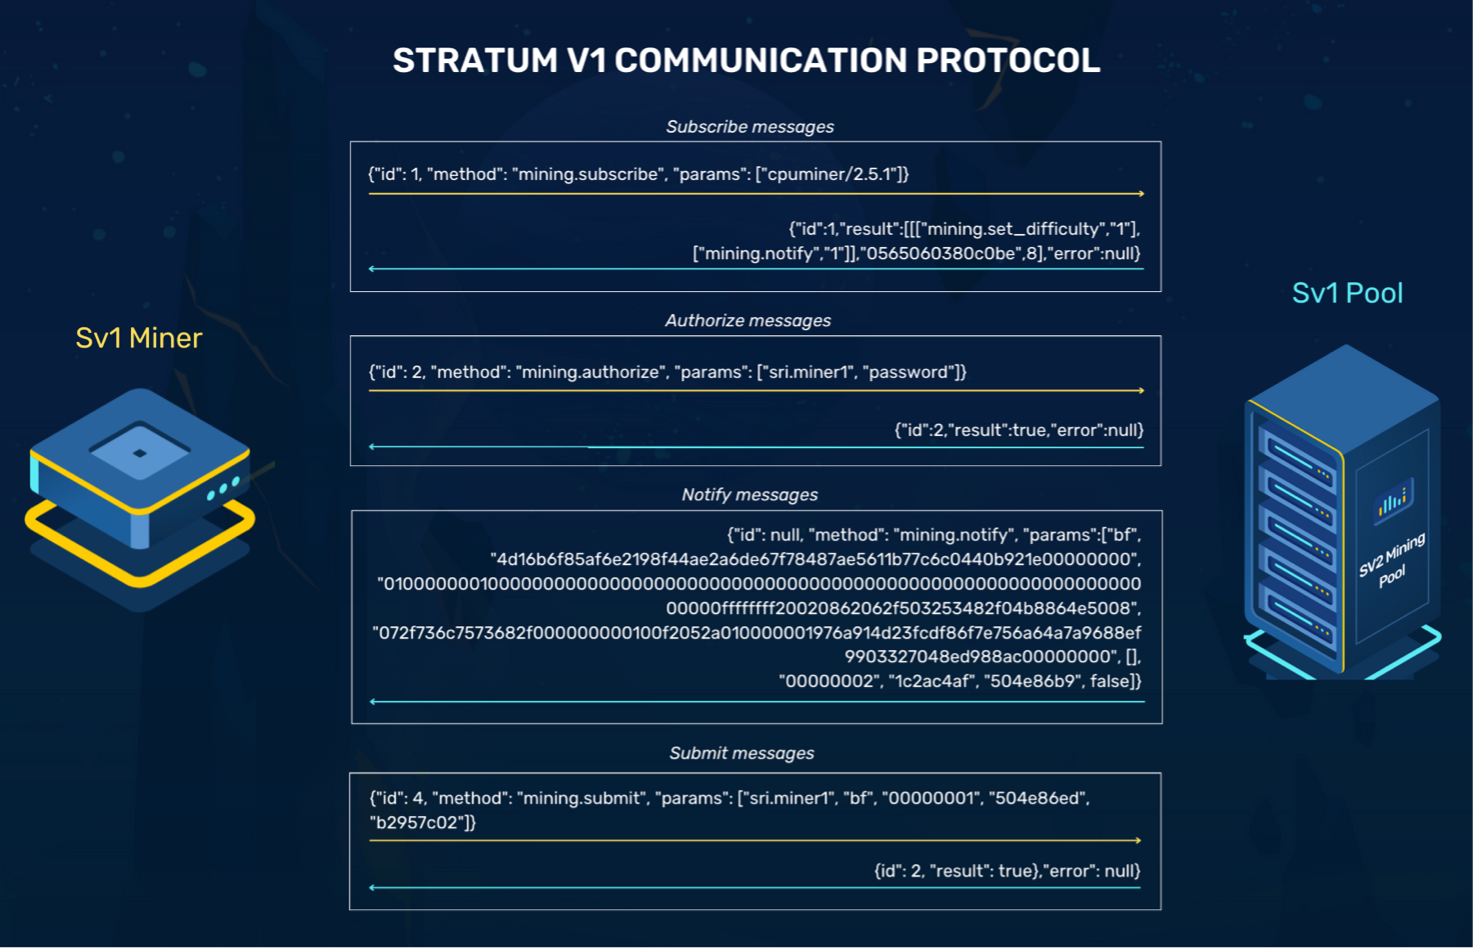
\includegraphics[width=15cm]{Figures/stratum/stratum2.png}
    \caption{Real communication between miner and pool server}
    \label{fig:stratum2}
\end{figure}